\documentclass[11pt,a4paper]{article}

\usepackage[utf8]{inputenc}
\usepackage[left=2cm,text={17cm, 24cm},top=3cm]{geometry}
\usepackage[T1]{fontenc}
\usepackage{graphics}
\usepackage{picture}

% =========================================================================
% BEGIN
% =========================================================================

\begin{document}

\begin{titlepage}

\thispagestyle{empty}

\begin{center}
  \LARGE
  \textsc{Brno University of Technology}\\
  \vspace{\stretch{0.382}}
  \medskip
  {\Huge NetFlow Security}\\
  \medskip
  {\LARGE SEC6NET}
  \medskip
  \smallskip
  \vspace{\stretch{0.618}}

{\Large Adam Štěpánek\hfill\today}

\end{center}

\end{titlepage}

\newpage


% =========================================================================
% UVOD
% =========================================================================

\section{Introduction}

The NetFlow architecture mainly consists of Exporter and Collector. Exporters listen to the network traffic and generate NetFlow records with the information of monitored network. Collector is generally a machine or a device where the records are sent to and stored. They can be later processed and viewed by the administrators for easy maintenance of the network.

As an exporter, either a specialized device or a computer with an installed software can be used. Specialized devices use custom hardware and so they are usually high performance. Software is supplied by the vendor and therefore it is not easy to make changes.

A computer with an installed software is not so high performance and is unable to process huge amounts of data as expensive special purpose devices. The advantage is that a custom solution can be made, especially as a piece of code running on Linux or FreeBSD operating system.

These exporters can be attached to the network by the Test Access Port (TAP) or the Switched Port Analyzer (SPAN) as seen in the Figure \ref{exporters}.

\begin{figure}[h]
  \begin{center}
    \scalebox{1.1}{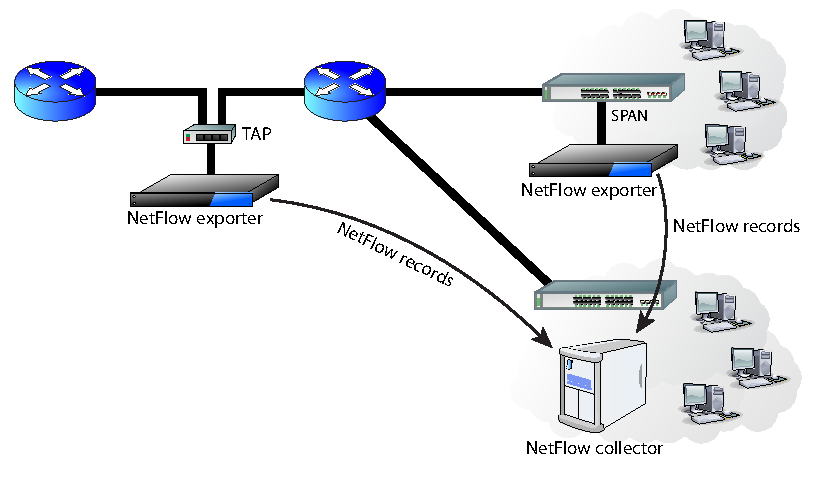
\includegraphics{fig/exporters.pdf}}
    \caption{NetFlow architecture with Exporter and Collector}
    \label{exporters}
  \end{center}
\end{figure}

Collector is usually a server with a high capacity storage where NetFlow records are kept. It is running a specialized software which allows to receive, store and presents records in a suitable form to administrators, including filtering by multiple criteria.

\section{Conceptual Solution of Secure Transport} 

Traditionally, data from an exporter to a collector is transfered by an unreliable channel. The situation is depicted in the Figure \ref{trad-arch}. Exporter creates a record and sends it to Collector. The unreliable channel is either repsented by a dedicated link or by any other infrastructure. It is the Internet in many cases. Data is transfered by the IP protocol which doesn't guarantee a reliable delivery. This is called best effort delivery and it is based upon the current network load. 

\begin{figure}[h]
  \begin{center}
    \scalebox{1.2}{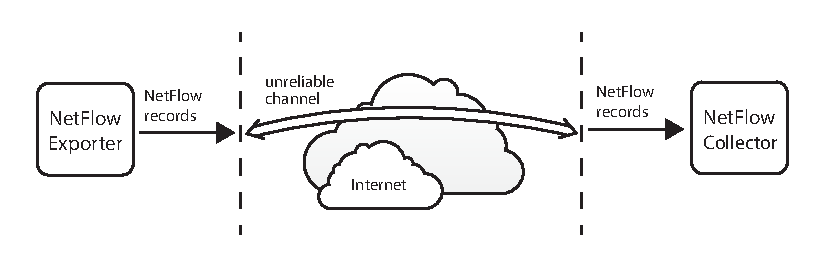
\includegraphics{fig/trad-arch.pdf}}
    \caption{Traditional architecture with the unreliable channel}
    \label{trad-arch}
  \end{center}
\end{figure}

The solution for the reliable delivery adds two components to the architecture: Sender and Receiver. Sender receives NetFlow records from Exporter and sends them securely to Receiver which creates original records and sends them further to Collector. If there is a failure in the connection between Sender and Receiver records are stored in the buffer in Sender. When the connection is re-established, records are sent and removed from the buffer. The architecture is depicted in the Figure \ref{reliable-arch}.

\begin{figure}[h]
  \begin{center}
    \scalebox{1.1}{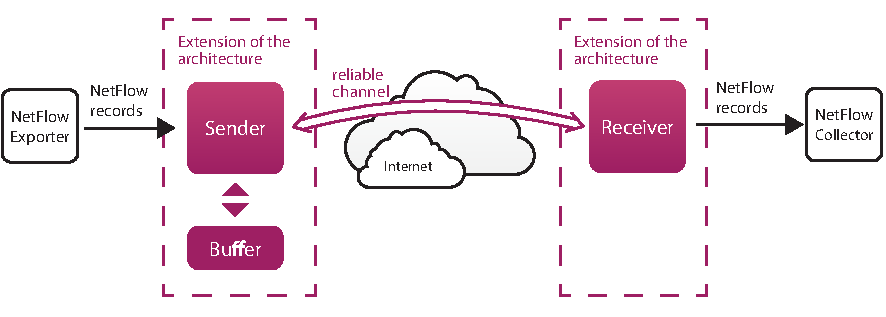
\includegraphics{fig/reliable-arch.pdf}}
    \caption{Reliable architecture with two components: Sender and Receiver}
    \label{reliable-arch}
  \end{center}
\end{figure}

Sender and Receiver don't need to be necessarily standalone components. Sender can be a part of the machine where Exporter resides as well as Receiver can be a part of the Collector device.

Regardless of the Sender and Receiver components, the architecture with reliable channel is the same as the traditional one. The physical channel stays untouched. The abstract reliable channel is made up of appropriate technics of communication and encapsulation of data transfered between Sender and Receiver. The whole solution is a noninvasive one and it is not necessary to make extensive alterations to the existing architecture.

\section{Implementation}

Conceptual Sender and Receiver are implemented, respectively, as \texttt{nf\textunderscore sender} and \texttt{nf\textunderscore receiver} daemons. Implementation language is Perl.

\subsection{Sender}

Sender consists of two threads: UPD server and TCP client. UDP server receives NetFlow records from the exporter and saves them to Buffer. TCP client picks up records from Buffer, sends them to Receiver and provides a general communication with Receiver.

Buffer as seen in the Figure \ref{reliable-arch} is represented by a directory \texttt{/tmp/flow.queue/} where the cache files are saved. A file is created every 5 minutes in the queue. When the connection to Receiver is working correctly the data is sent immediately to Receiver. If the connection fails the queue files are stored on the sender's side until a new connection is established. Subsequently, the data to Receiver are sent in the same order as were previously received from the NetFlow probe.

\subsection{Receiver}

Receiver has only one thread. It ensures receiving of NetFlow records and passing them to the collector.

\subsection{Communication}

If the connection between Sender and Receiver fails, Sender tries to re-establish the connection after one second. Every next unsuccessful attempt makes the time three times longer, ie. three seconds, nine seconds, twenty seven seconds and so on. Maximum waiting time is 243 seconds. It means once in 243 seconds Sender tries to establish the connection to Receiver until it succeeds.

The communication can be optionally encrypted with a shared key using the Blowfish cipher. For this purpose the option \texttt{-k <key>} have to be set to the same value on both sides. If the keys don't match Receiver refuses to accept the data and these are kept in the queue. However, the data in the queue is kept unencrypted.

\section{Installation and Usage}

Both \texttt{nf\textunderscore sender} and \texttt{nf\textunderscore receiver} daemons are distributed in a single source RPM package from which two RPMs are generated: for \texttt{nf\textunderscore sender} and \texttt{nf\textunderscore receiver}. Steps for the installation depends on the distribution you use. For more information type: \texttt{man rpm}.

When the installation is complete, navigate to \texttt{/etc/sysconfig/} and edit the files \texttt{nf\textunderscore sender} and \texttt{nf\textunderscore receiver} according to the instructions in them. These configuration files set the options for running daemons in your desired configuration. If not set, default options will be used. For more information about the available options, see manual pages (type \texttt{man nf\textunderscore sender} or \texttt{man nf\textunderscore receiver}).

In order to start the daemons, you can either reboot your computer and the daemons will start automatically or you type \texttt{/etc/init.d/nf\textunderscore sender start} and \texttt{/etc/init.d/nf\textunderscore receiver start}. The same way you start the daemons, you can stop them using the word \texttt{stop} instead of \texttt{start}. You can also restart the daemons using the word \texttt{restart}. 

\end{document}
